\documentclass[10pt,a4paper]{article}
\usepackage[utf8]{inputenc}
\usepackage{amsmath}
\usepackage{amsfonts}
\usepackage{amssymb}
\usepackage{graphicx}
\usepackage{verbatim}
\usepackage[margin=1in]{geometry}

\setlength\parindent{0pt} % Removes all indentation from paragraphs

\author{Nikola Janju\v{s}evi\'{c}}
\title{ECE471, Selected Topics in Machine Learning \\ Assignment 2}
\date{September 11, 2018}

\begin{document}
\begin{large}
ECE471, Selected Topics in Machine Learning -- Assignment 2
\end{large} \\
Nikola Janju\v{s}evi\'{c} \\
September 11th 2018 

\subsubsection*{Remarks}
This assignment called for binary classification of "spiral data". This data is generated in the code below and represented by as blue and red dots in Figure 1. A multi-layer perceptron (MLP) was trained by this data to produce a conditional pdf determining the probability that a point is in class t=1 (the red dots). It takes in 2D Cartesian coordinates and outputs logits. The following remarks were noted during this process:
\begin{itemize}
\item smaller batch sizes can give faster convergence
\item relu6 achieves much better results as an activation function than the sigmoid.
\item using 2 MLP layers gave noticeably better performance over 3 layers
\item keeping the output layer as a linear combination yielded better results
\item a batch size greater than the number of parameters in the first layer yeilds better results
\end{itemize}
Initially, it took \verb|50,000| batches to achieve usable results and have a (personal) proof of concept of the MLP. The remarks above are a result of tuning that initial design. Specific to this machine learning problem, it was found that the MLP could produce decent results with \verb|1000| batches, but this often left some undesired miss-classification in the spiral paths. 
\begin{verbatim}
import matplotlib.pyplot as plt
import numpy as np
import tensorflow as tf
from numpy.random import *
import time
from tqdm import tqdm

# intermediate dimensional number
M = 40
dim_in = 2
dim_layer1 = M
dim_layer2 = M
BATCH_SIZE = 2*M
NUM_BATCHES = 5000

class Data(object):
    def __init__(self):
        seed(int(time.time()))
        # number of samples is really twice this
        nsamp = 300
        self.index = np.arange(2*nsamp)

        var = .1
        # noise
        v = np.sqrt(var/2)*randn(nsamp,4)

        # class 0
        t1 = uniform(np.pi/4, 4*np.pi, nsamp)
        x1 = np.array([ t1*np.sin(t1)+v[:,0], t1*np.cos(t1)+v[:,1] ]).T

        # class 1
        t2 = uniform(np.pi/4, 4*np.pi, nsamp)
        x2 = np.array([ -t2*np.sin(t2)+v[:,2], -t2*np.cos(t2)+v[:,3] ]).T

        self.x = np.concatenate((x1,x2))
        self.y = np.concatenate((np.zeros(nsamp), np.ones(nsamp)))

    def get_batch(self):
        choices = choice(self.index, size=BATCH_SIZE)
        return self.x[choices,:], self.y[choices].flatten()

# Store layers weight & bias
# default dtype=float32
weights = {
    'w1': tf.Variable(tf.random_normal([dim_in, dim_layer1])),
    'w2': tf.Variable(tf.random_normal([dim_layer1, dim_layer2])),
    'out': tf.Variable(tf.random_normal([dim_layer2, 1]))
}
biases = {
    'b1': tf.Variable(tf.random_normal([dim_layer1])),
    'b2': tf.Variable(tf.random_normal([dim_layer2])),
    'out': tf.Variable(tf.zeros([]))
}

# f:R2 -> R
def f(x):
    # R2 -> Rdim_layer1
    layer_1 = tf.nn.relu6(
        tf.add( tf.matmul(x, weights['w1']), biases['b1'] )
    )
    # Rdim_layer1 -> Rdim_layer2
    layer_2 = tf.nn.relu6(
        tf.add( tf.matmul(layer_1, weights['w2']), biases['b2'] )
    )
    # Rdim_layer2 -> R
    return tf.squeeze(
            tf.add( tf.matmul(layer_2, weights['out']), biases['out'] )
    )

x = tf.placeholder(tf.float32, [None,2])
y = tf.placeholder(tf.float32, [None])
logits = f(x)

# binar cross entropy loss with L2 penalty on weights
loss = tf.reduce_mean( tf.losses.sigmoid_cross_entropy(y, logits) ) + \
    (.05/M**2)*tf.reduce_sum( [tf.nn.l2_loss(var) for var in
        tf.get_collection(tf.GraphKeys.TRAINABLE_VARIABLES)] )
optim = tf.train.GradientDescentOptimizer(learning_rate=0.1).minimize(loss)
init = tf.global_variables_initializer()

with tf.Session() as sess:
    data = Data()
    sess.run(init)
    # training
    avg_cost = 0.;
    for _ in tqdm(range(0, NUM_BATCHES)):
        x_np, y_np = data.get_batch()
        loss_np, _ = sess.run([loss, optim], feed_dict={x: x_np, y: y_np})
        avg_cost  += loss_np/NUM_BATCHES
    print("cost={:.9f}".format(avg_cost))

    # prediciton
    pred = tf.nn.sigmoid(logits)
    # meshgrid resolution
    N = 150
    xx = np.linspace(-15, 15, N)
    X1,X2 = np.meshgrid(xx,xx,indexing='ij')
    P = np.zeros( (N,N) )
    for i in range(N):
        for j in range(N):
            xp = np.array([ X1[i,j], X2[i,j] ]).reshape(1,2)
            P[i,j] = sess.run(pred, feed_dict={x: xp})

    plt.figure()
    data_c1 = data.y>.5
    data_c0 = data.y<.5
    plt.plot(data.x[data_c1,0], data.x[data_c1,1],
        'or', markeredgecolor="black")
    plt.plot(data.x[data_c0,0], data.x[data_c0,1],
        'oc', markeredgecolor="black")
    plt.pcolor(X1,X2,P, cmap="coolwarm")
    plt.xlabel("x1")
    plt.ylabel("x2")
    plt.legend(["class: t=1", "class: t=0"])
    cb = plt.colorbar()
    cb.set_label("p(t=1 | x)", rotation=0)
    plt.title("multilayer perceptron generated pdf \nwith training data")
    plt.show()
\end{verbatim}

\begin{figure}[h]
\centering
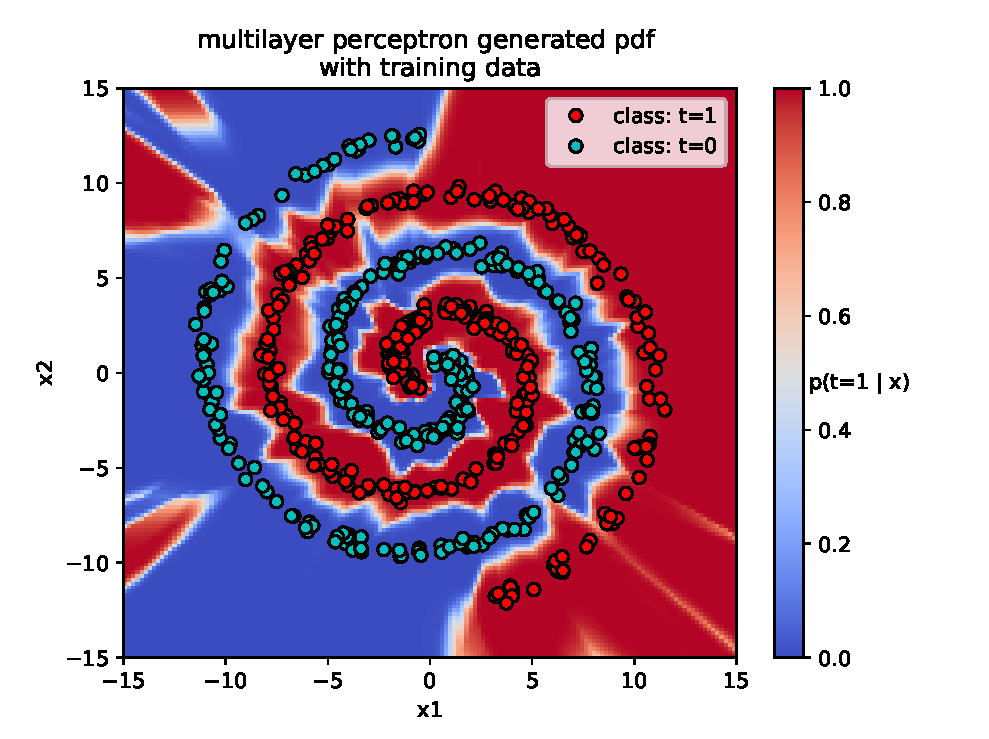
\includegraphics[width=\textwidth]{Figure_1.pdf}
\caption{Conditional PDF of the MLP (color-gradient) superimposed with the training data}
\end{figure}

\end{document}